
Este capítulo apresenta, inicialmente, os detalhes do módulo de escalonamento do BioNimbuZ. Posteriormente, discorre sobre a implementação, mostrando alguns dos problemas encontrados durante o desenvolvimento e como eles foram solucionados. A terceira seção aborda a adição de tarefas que utilizam a \acrshort{GPU} no BioNimbuZ, e na última parte deste capítulo são descritos os testes que podem ser feitos e o resultados obtidos a partir do novo escalonador.

\section{Sistema de Escalonamento do BioNimbuZ}

O Serviço de Escalonamento é implementado no BioNimbuZ como um serviço da Camada de Núcleo (veja a Figura \ref{Arquitetura}), de acordo com o subsistema mostrado na Figura \ref{SubsistemaDeEscalonamento}. A interface \textit{services} define métodos para a inicialização, o término de serviços e os métodos para comunicação com o \textit{Zookeeper} \cite{Zookeeper}. 
\begin{figure}[htbp]
	%	\centerline{\includegraphics[scale=0.04]{img/EscalonadorProposto.png}}
	\centerline{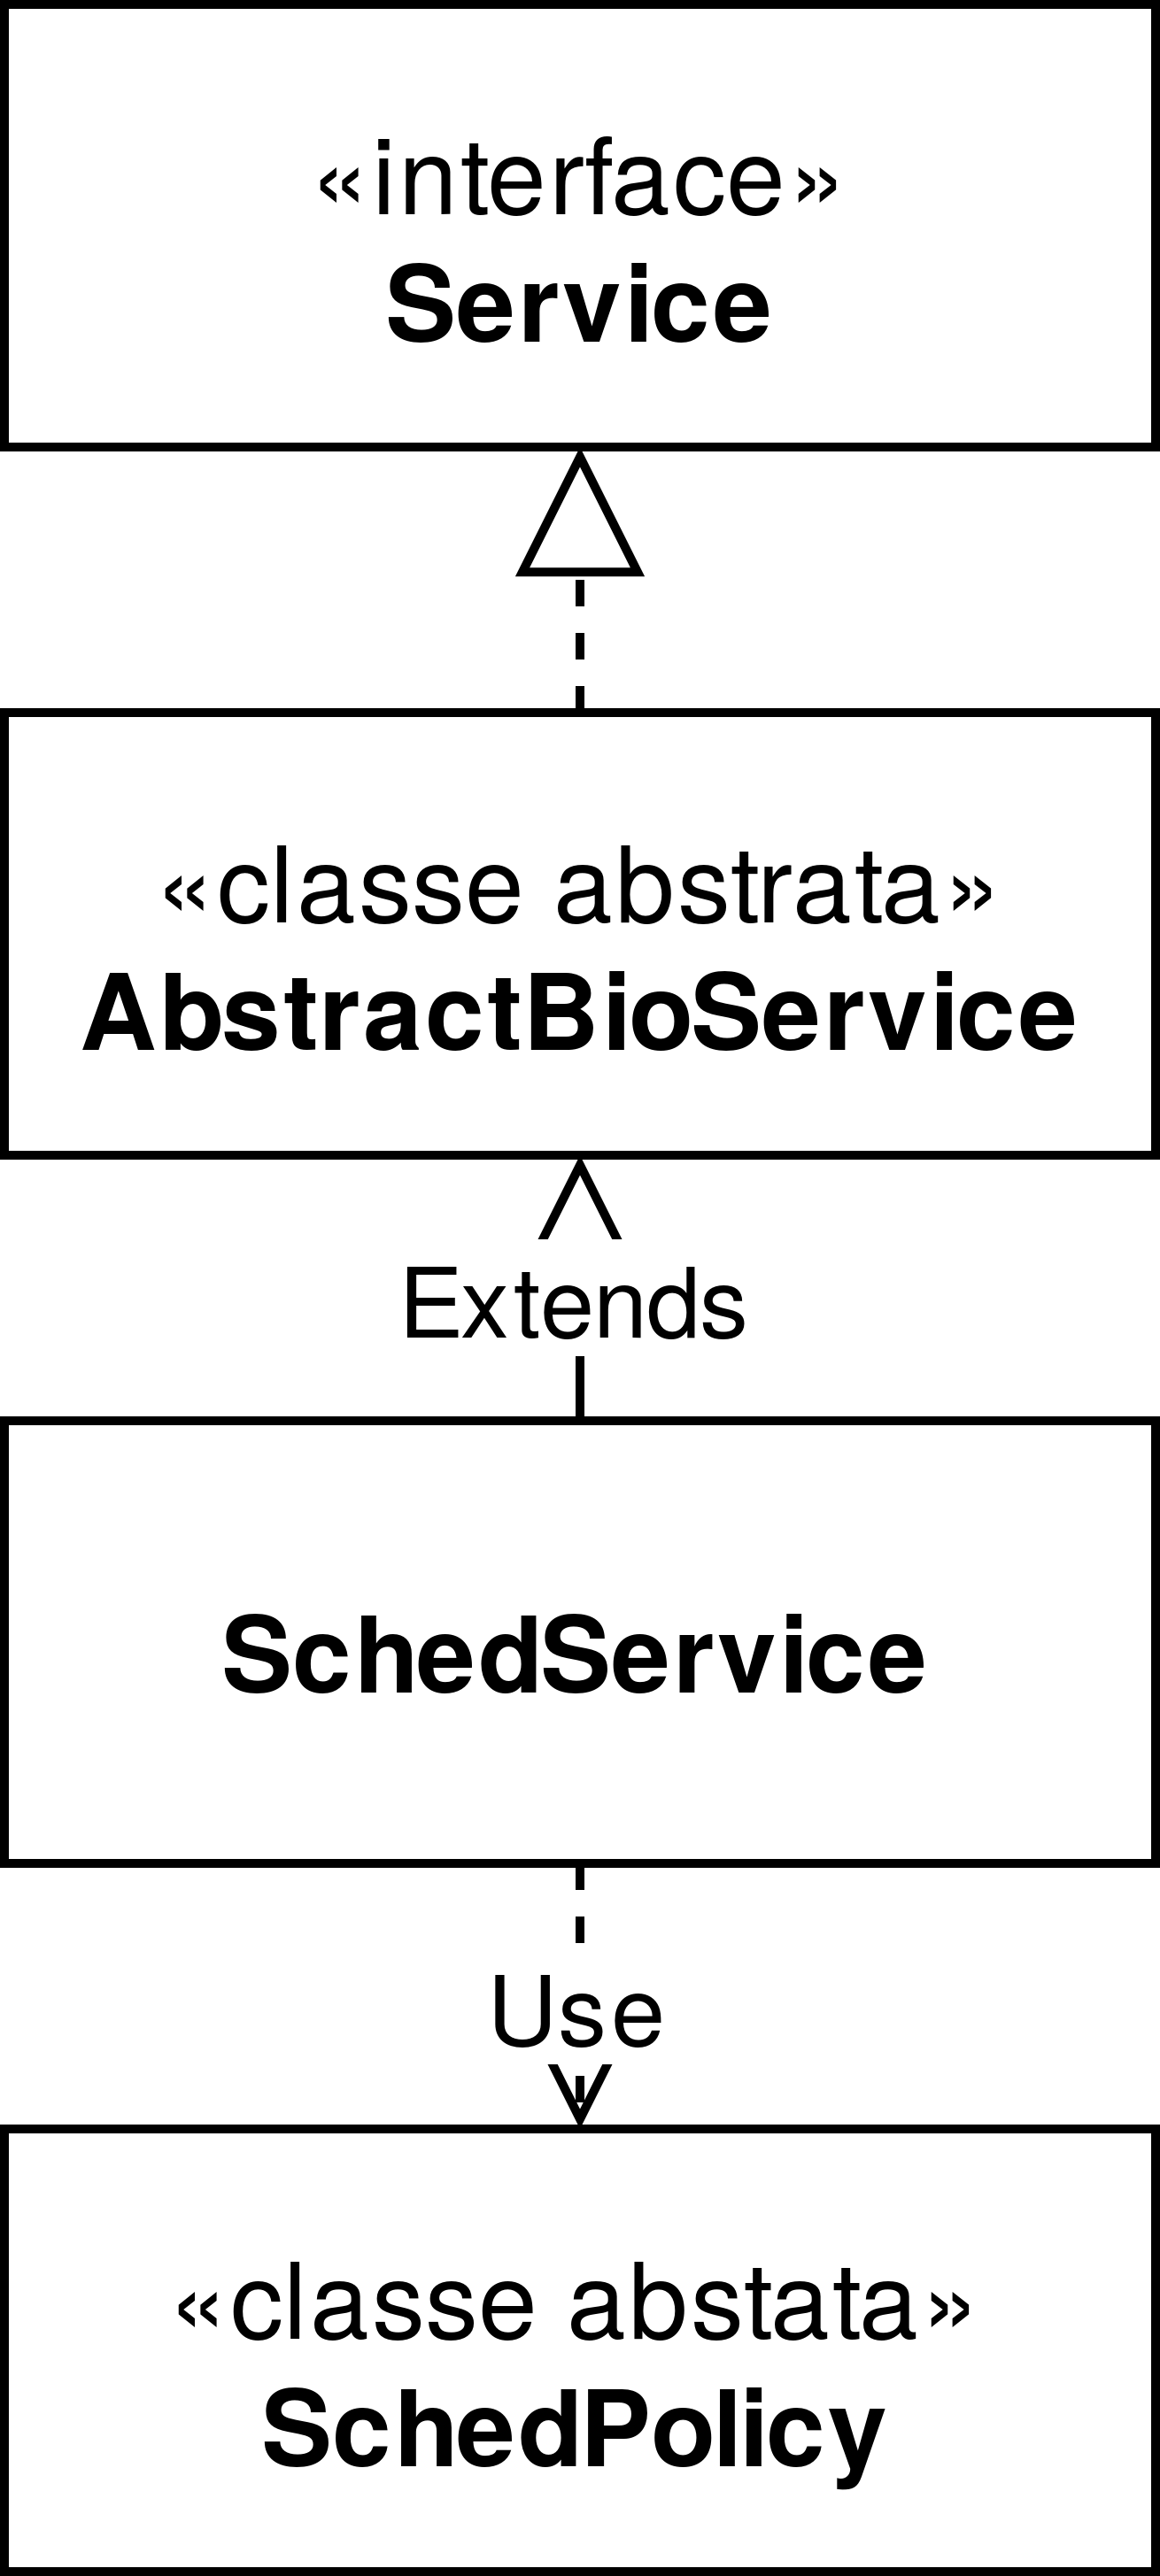
\includegraphics[width=2.8cm]{img/SubsistemaDeEscalonamento.png}}
	\caption{Subsistema de Escalonamento do BioNimbuZ.}
	\label{SubsistemaDeEscalonamento}
\end{figure}
A classe \textit{AbstractBioService} define funcionalidades comuns aos serviços do BioNimbuZ, em especial, a comunicação entre as máquinas que compõem a plataforma e o padrão de projeto \textit{observer}, utilizado para notificação de eventos.

A classe \textit{SchedService} é a responsável por prover o serviço de escalonamento em si, entretanto, para permitir a existência de várias políticas de escalonamento, internamente ela utiliza instâncias da classe abstrata \textit{SchedPolicy}, que implementam cada uma das distintas políticas de escalonamento existentes, conforme mostrado na Figura \ref{ArquiteturaAtual}.

Essas políticas de escalonamento são implementadas por meio da definição dos seguintes métodos herdados de \textit{SchedPolicy}:
\begin{itemize}
%	\item \textit{schedule}, que recebe como arguento uma lista de \textit{Jobs} para ser escalonado e retorna um mapeamento de \textit{Job} para um conjunto de máquinas as quais realizarão a computação.
	\item \textit{schedule}, que realiza o escalonamento inicial propriamente dito;
	\item \textit{relocate}, o qual realoca um processamento que está em execução;
	\item \textit{cancelJobEvent}, cujo objetivo é reportar ao escalonador o cancelamento de um \textit{job};
	\item \textit{jobDone}, que informa ao escalonador que um \textit{job} terminou.
\end{itemize}

\begin{figure}[htbp]
	\centerline{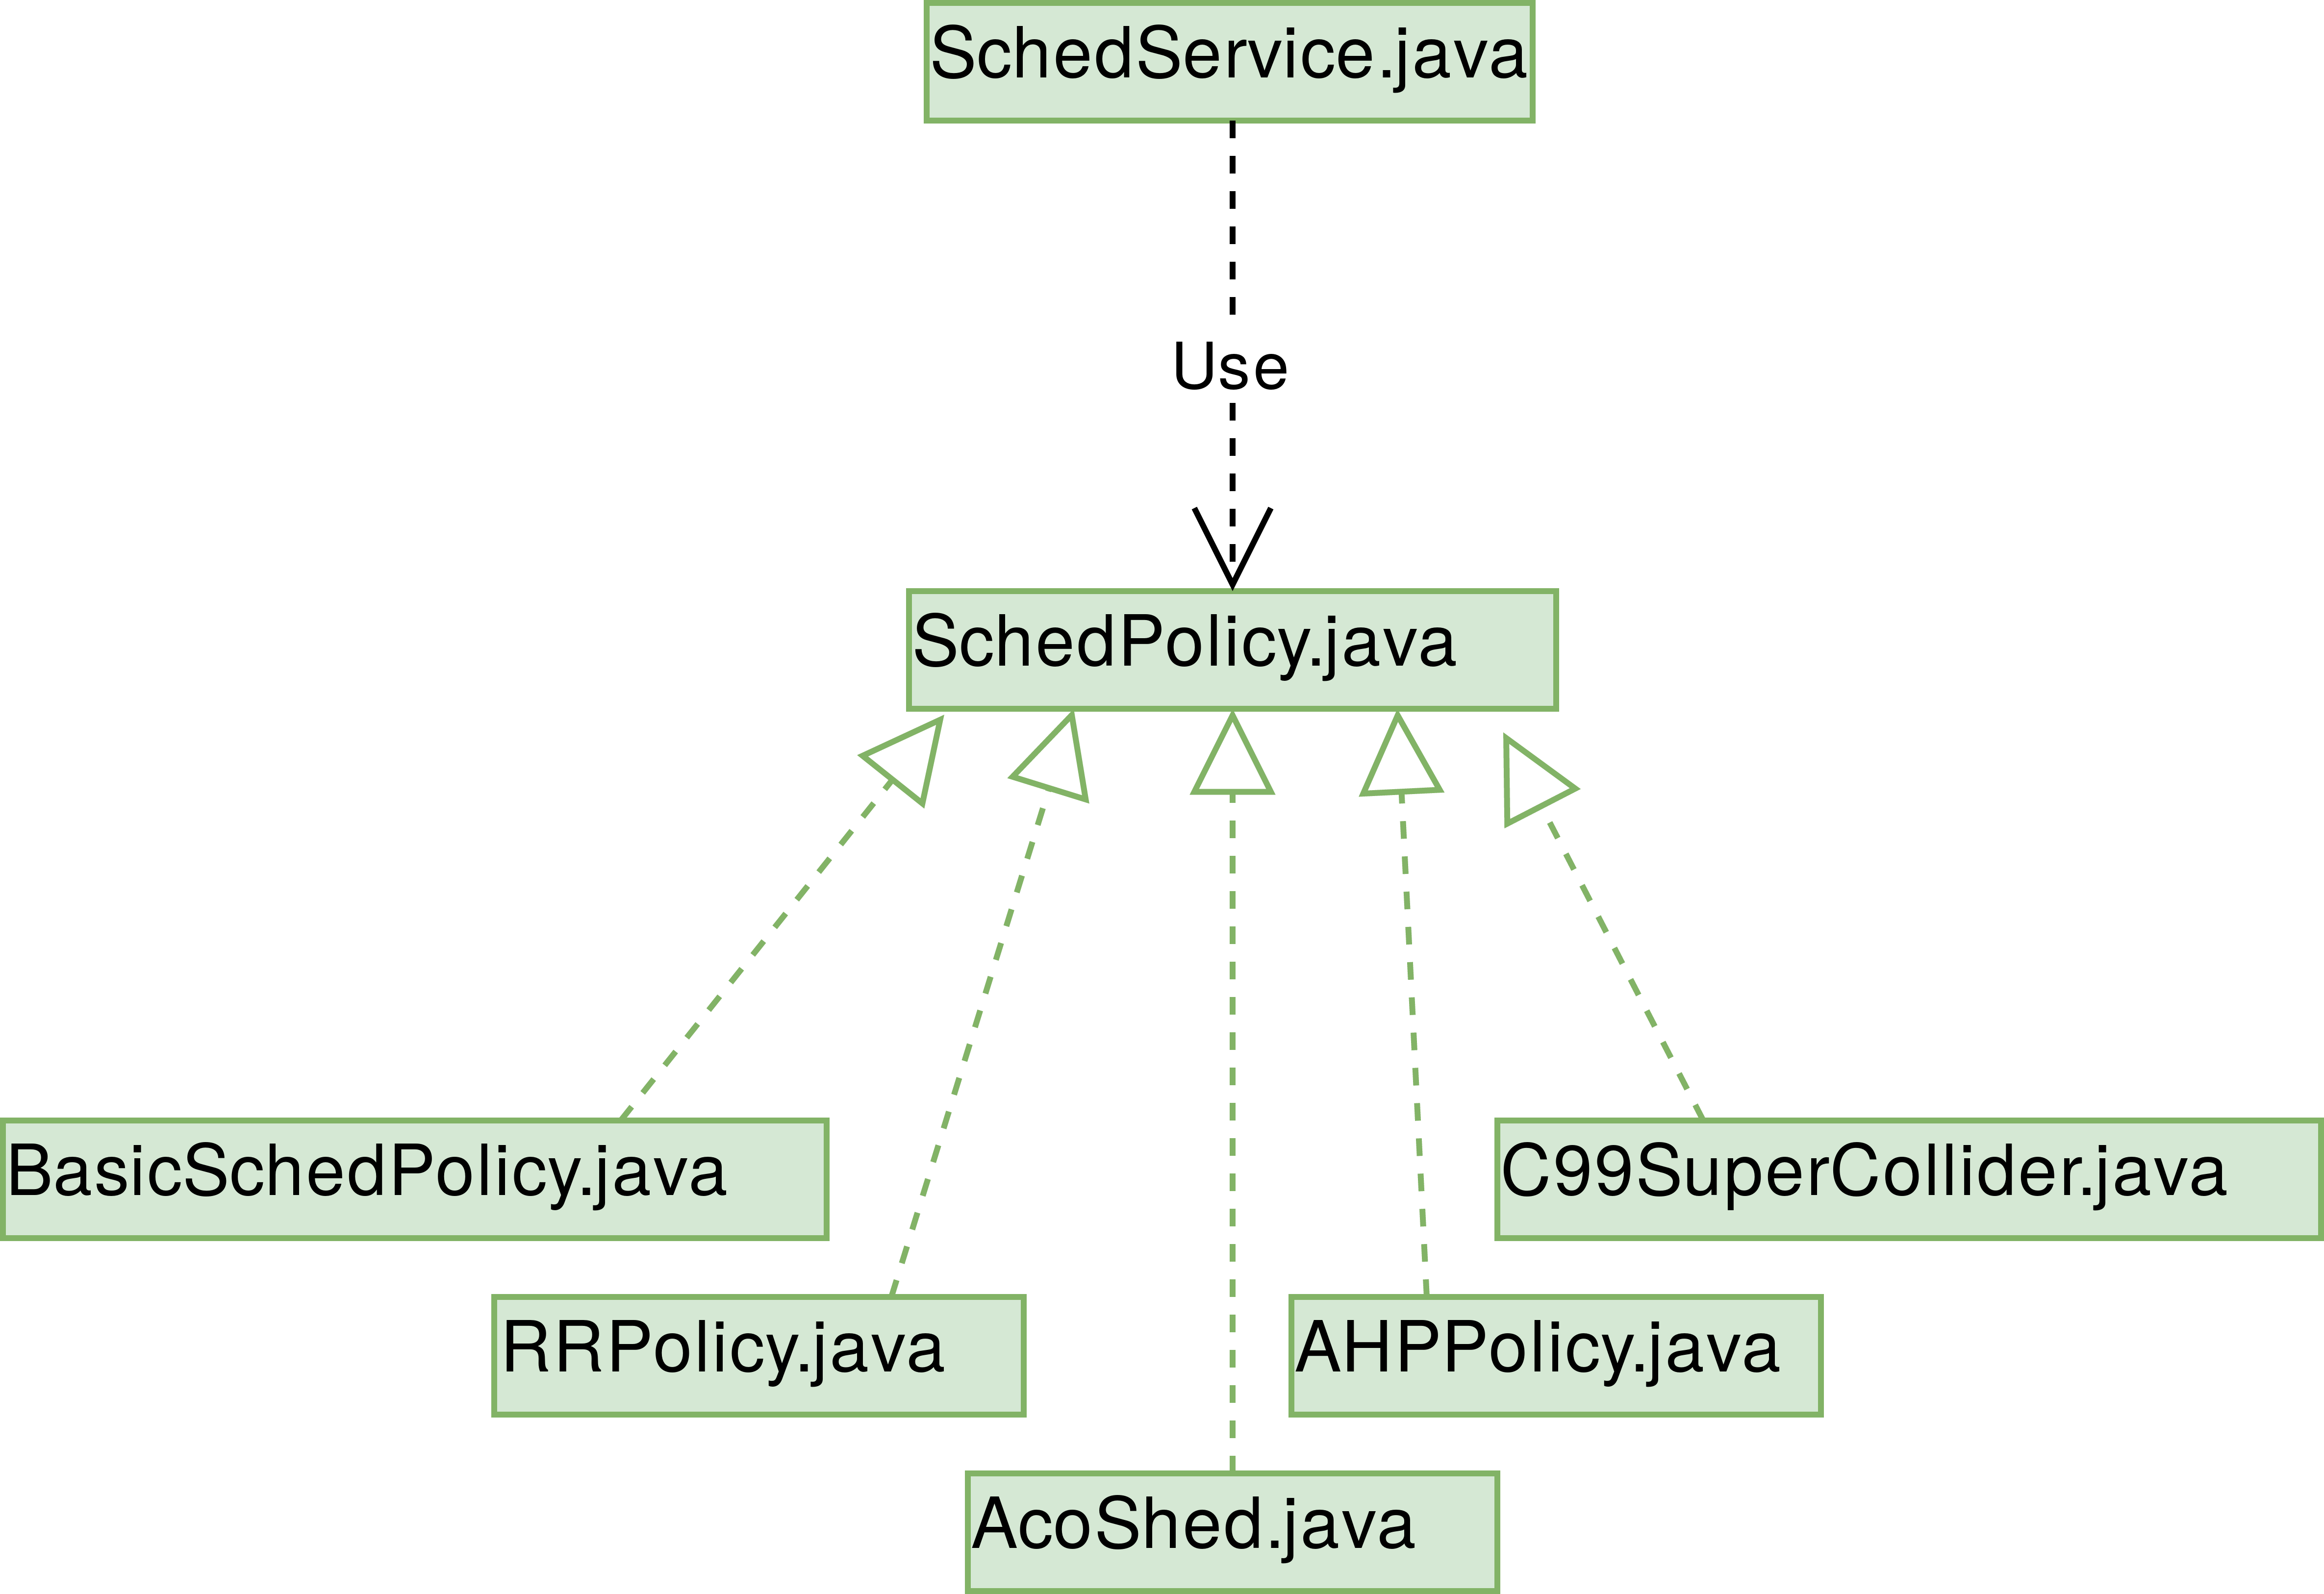
\includegraphics[width=12cm]{img/ArquiteturaAntesHoriz.png}}
	\caption{Subsistema de Escalonamento do BioNimbuZ.}
	\label{ArquiteturaAtual}
\end{figure}


\section{Implementação do Escalonador Proposto}

Por motivos de familiaridade com a linguagem de programação, o escalonador proposto foi implementado em C++. Para ter compatibilidade com os demais componentes do software, classes auxiliares, como a que representa os \textit{Jobs} e as \acrshort{VM}s instanciáveis tiveram equivalentes escritos em C++. Além disso, dois outros problemas surgiram, que foram como iniciar o escalonador C++, e como ele deve se comunicar com os demais componentes da plataforma. O primeiro problema foi resolvido por meio de pesquisa na \acrfull{API} do Java, utilizando as classes \textit{Process}\cite{JavaProcess}, \textit{Runtime}\cite{JavaRuntime} e \textit{ProcessBuilder}\cite{JavaProcessBuilder}, os quais permitem executar comandos de terminal, o que possibilitou a execução da parte C++ do escalonador.

O problema da comunicação do C++ com o Java é mais difícil, pois há várias formas de fazer. Por exemplo, o uso de classes \textit{wrappers} que usam \textit{handles}, que são objetos cujo objetivo é manipular estruturas que não são nativas da linguagem\cite{CppJavaHandle}. Uma outra forma documentada é através do uso do \acrfull{JNI}, que é uma outra forma existente no qual, através do uso de \textit{handles}, é chamado o código C++ num programa Java\cite{CppJavaJNI}. Além disso, existem variações deste método utilizando bibliotecas que buscam simplificar o gerenciamento do \textit{handle}. Como as formas pesquisadas para fazer tal comunicação aparentam não chegar a um consenso, decidiu-se então utilizar formas mais genéricas de comunicação entre processos, o qual surgiu a ideia de usar \textit{sockets} para fazer a comunicação.

\textit{Socket} é uma abstração que sistemas operacionais fazem para permitir que programas tenham acesso à rede. \iffalse Os sistemas operacionais organizam os \textit{sockets} disponíveis e portas, essa organização de portas também é utilizada por protocolos de rede, \fi O sistema de portas permite diferenciar em um computador qual dos programas interessados está enviando ou deve receber a mensagem. %E um truque que pode ser feito usando a pilha de rede \acrshort{TCP/IP} é enviar mensagens para o próprio computador, através da interface de rede de \textit{loopback}. E esse é um método efetivo de comunicação entre processos distintos.

\begin{figure}[htbp]
	\centerline{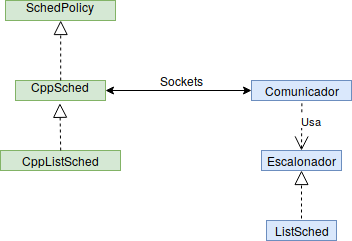
\includegraphics[scale=0.7]{img/Proposta.png}}
	\caption{Arquitetura de Classes do Escalonador Implementado.}
	\label{ArquiteturaProposta}
\end{figure}

Uma vez decidido o uso de \textit{sockets}, faltava decidir qual seria o protocolo da camada de rede e de transporte. Na camada de rede o principal protocolo existente é o \acrfull{IP}, entretanto, existem duas versões: o IPv4\cite{ipv4rfc} e o IPv6\cite{ipv6rfc}, sendo que o último é mais recente e permite um maior número de dispositivos na rede, por isso essa foi a versão utilizada na implementação. Quanto à camada de transporte, os candidatos eram o \acrshort{TCP}\cite{tcp_rfc} e o \acrshort{UDP}\cite{udp_rfc}. O \acrshort{TCP} provê uma série de garantias ao usuário dos pacotes que serão transmitidos pela rede ao custo de \textit{overhead}, mas como apenas será utilizado para comunicação em \textit{loopback}. O \acrshort{UDP} é mais simples e enxuto, sendo o escolhido como protocolo da camada de transporte neste trabalho.

%Uma dificuldade encontrada durante a implementação do uso de \textit{sockets}, foi como utilizar o IPv6, pois, especialmente para a linguem C, há pouca documentação disponível sobre, por mais que exista boa documentação sobre o uso de \textit{sockets} IPv4.


Como pode ser observado na Figura \ref{ArquiteturaProposta}, para a implementação desse sistema de comunicação no BioNimbuZ, desenvolveu-se a classe abstrata \textit{CppSched} que herda de \textit{SchedPolicy}, responsável por fazer a inicialização do programa C++ e pelo \textit{handshake} entre os processos C++ e Java, permitindo que futuros escalonadores em C++ não precisem repetir este processo. Da classe \textit{CppSched} herda o método \textit{GetSchedPolicy}, utilizado para informar qual escalonador C++ deve ser utilizado.

\begin{figure}[htbp]
	\centerline{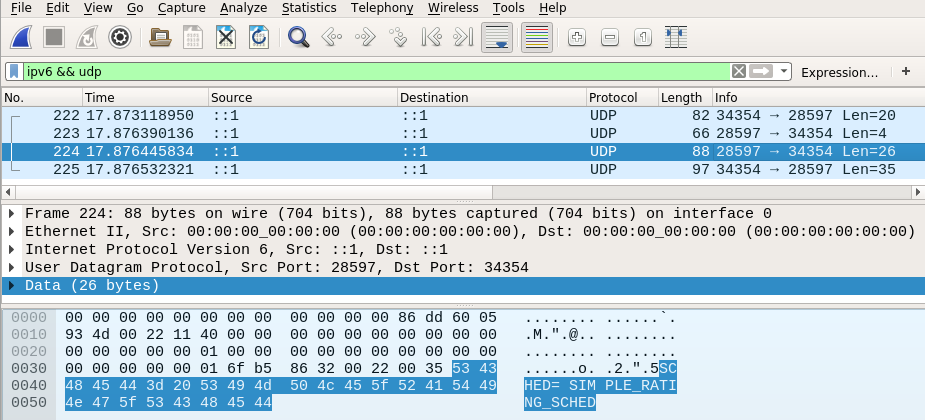
\includegraphics[width=13cm]{img/Handshake3.png}}
	\caption{Handshake entre a parte Java e C++ do Escalonador.}
	\label{Handshake}
\end{figure}

O programa C++ é composto pela classe Comunicador, que inicializa seu \textit{socket} e inicia a conversa com o processo Java, cuja porta de comunicação é recebida pela linha de comando. Durante o \textit{handshake} é definido qual filho da classe virtual Escalonador será usado. Em prol da simplicidade e da performance, buscou-se minimizar a comunicação entre os processos C++ e Java. Assim, após a inicialização, o processo C++ se comporta similarmente à um servidor \acrshort{DNS}\cite{dns_rfc}, ficando em espera por solicitações de escalonamento, e responde às requisições sem manter estado internamente.

\section{Aplicação Testada no BioNimbuZ}

%No início do projeto, imaginava-se que os \textit{workflows} existentes no BioNimbuZ seriam capazes de tirar proveito da \acrshort{GPU}, pressuposto que se revelou falso ao longo do desenvolvimento do projeto. Logo fez-se necessário procurar por programas de uso geral que utilizem a \acrshort{GPU}, uma atividade que se revelou simples. 
Para os testes foi escolhido o programa XMR-Stak\cite{xmr_stak}, um programa de mineração de criptomoedas, que são artefatos digitais desenvolvidos como meio de troca, que utilizam criptografia para prover segurança e integridade à transações\cite{crypto_currencies}. Esse software de mineração, em específico, foi escolhido pelo fato de ser software livre e, por isso, ter seu código fonte disponível publicamente, além de ser multiplataforma e capaz de executar tanto em \acrshort{CPU} quanto em acrshort{GPU}.

A mineração de criptomoedas é a atividade de buscar \textit{nouces}, isto é, uma sequência aleatória de bytes, que quando inserido junto de um possível futuro bloco de uma \textit{blockchain}, que é uma lista distribuída para armazenamento de registros, numa função de \textit{hash} criptográfico, gera um \textit{hash} que atenda a algum critério de dificuldade, geralmente um valor específico no início. Quando é encontrado um \textit{digest}, uma saída da função de \textit{hash}, que atende ao critério, tal bloco é adicionado na \textit{blockchain}, e o responsável pela máquina que encontrou a resposta é recompensado em criptomoeda.

Assim, uma vez testado a plataforma na \acrshort{VM}, é hora de testar em equipamento real, pois as máquinas virtuais não possuem acesso à \acrshort{GPU}, a não se quando utilizado \textit{\acrshort{GPU} Passthrough}, que é uma técnica que permite redirecionar o controle de uma \acrshort{GPU} física para uma máquina virtual. Uma das maiores barreiras para o \textit{\acrshort{GPU} Passthrough} é que ele requer pelo menos duas placas de vídeos, pois tanto o sistema hóspede quanto o sistema hospedeiro devem ter cada um sua \acrshort{GPU}.

%\subsection{Da \acrshort{VM} para a máquina de testes}

Após a plataforma apresentar correto funcionamento, toda a instalação seria clonada num \textit{flash drive} \acrshort{USB} capaz de inicializar, para tal o \textit{bootloader}, \textit{software} responsável por determinar como o sistema será inicializado, ser reparado para que seja capaz de inicializar a partir do dispositivo móvel de armazenamento. O sistema precisa ser clonado pois usa pacotes de versões diferentes do sistema operacional Debian\cite{Debian}, porque o XMR-Stak utiliza a biblioteca de processamento paralelo \acrshort{CUDA}\cite{CUDA}, da Nvidia\cite{NVIDIA},e essa biblioteca requer o uso da versão 6 do compilador \acrshort{GCC}\cite{GCC}, disponível no repositório da versão \textit{stable} do Debian. A biblioteca do CUDA está disponível na versão \textit{unstable} do sistema operacional. O \acrshort{CUDA} foi retirado da versão \textit{testing} do Debian por causa dessa dependência da versão 6 do \acrshort{GCC}, que é considerada desatualizada\cite{CUDA_BUGREP}.


\section{Implantação no BioNimbuZ}

O escalonador foi, inicialmente, desenvolvido utilizando apenas o subsistema de escalonamento do BioNimbuZ, para que testes fossem feitos com rapidez. Após testes que comprovaram o funcionamento do escalonador, como o da Figura \ref{Handshake}, utilizou-se uma máquina virtual para fazer a implantação do escalonador desenvolvido de volta ao BioNimbuZ, pois a instalação do BioNimbuZ requer instalação de programas que podem, mesmo que seja incomum, conflitar ou apresentar erros em iterações com o resto do sistema operacional. Um exemplo que ocorreu durante o desenvolvimento foi uma atualização do sistema operacional, Debian\cite{Debian} Testing\cite{DebianTesting}, que causou erros em tempo de execução no \acrfull{IDE} Eclipse\cite{JavaEclipse}, relativos à interface gráfica. O mecanismo de \textit{snapshots} providos pelo software de gerenciamento de \acrshort{VM}s Virtualbox\cite{VirtualBox} se revelou realmente útil nessa circunstância, como pode ser visto na Figura \ref{Snapshots}.

\begin{figure}[htbp]
	\centerline{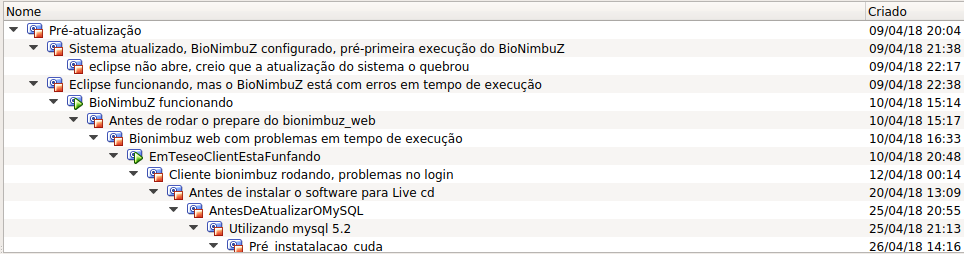
\includegraphics[width=12cm]{img/Snapshots.png}}
	\caption{Parte dos \textit{Snapshots} existentes na \acrshort{VM} de Implantação.}
	\label{Snapshots}
\end{figure}

Nos primeiros testes de funcionamento do BioNimbuZ, percebeu-se um erro no qual era possível cadastrar novo usuários, mas não era possível logar na plataforma, apenas aparecendo a mensagem "Erro Interno". Pesquisa nos arquivos de \textit{log} mostraram que o BioNimbuZ não estava conseguido criar a maioria de suas tabelas no \acrfull{SGBD} MySQL, devido ao tamanho de limite de linha das tabelas, causado pele junção de vários campos para armazenamento de \textit{strings} e o fato do \acrshort{SGBD} utilizar 4 bytes para codificar cada caractere. Após pesquisar possíveis soluções, incluindo atualização do MySQL, decidiu-se criar manualmente as tabelas que apresentavam esse problema, reduzindo o tamanho de alguns campos de texto, solução que resolveu o problema sem perda aparente de funcionalidade.

Outro problema enfrentado durante o desenvolvimento foi que \textit{workflows} não eram enviados para execução quando solicitado, os \textit{logs} apenas informavam "Error: NULL", sem maiores informações para solucionar o problema, que foi identificado como uma inicialização incompleta do BioNimbuZ por causa que a \textit{thread} que inicializava a plataforma ficava à espera de uma mensagem que já havia sido recebida no \textit{socket}, porém incorretamente descartado porque no Java, para se comparar a mensagem recebida com o que se espera, é necessário explicitar a codificação tanto da mensagem recebida quando do texto esperado.

Mais uma adversidade ocorrida durante a implantação é que quando se seleciona o computador local para executar uma tarefa, esse computador não é listado entre as máquinas disponíveis para o escalonamento. Assim, nenhuma outra máquina for escolhida para escalonamento, a requisição que o escalonador recebe não disponibiliza máquinas para escalonar, fazendo com que o escalonamento falhe. O falha que causou esse erro está relacionada com a visibilidade do mapa de nuvens disponíveis na hierarquia de classes, uma vez encontrada a forma correta de acesso à essa informação o problema foi resolvido.

Com o problema acima resolvido, o escalonamento estava funcionando corretamente, porém o BioNimbuZ não inicializava o \textit{Job} do minerador alegando a falta de um arquivo de entrada de nome vazio e sem informações sobre, por mais que o minerador em si não necessitasse. Após compreender que esse problema está relativo ao fato de o BioNimbuZ trabalhar com \textit{workflows}, para os quais é suposto a existência tanto de entrada, quanto de saída. A solução de contorno para esse problema foi simplesmente informar colocar um arquivo qualquer como entrada para o XMR-Stak no BioNimbuZ.

Após todos esses problemas terem sido resolvidos, percebeu-se que o \textit{software} modifico de mineração XMR-Stak estava falhando em sua inicialização, descobriu-se então que a criptomoeda utilizada para a mineração teve seu algoritmo de mineração modificado e então foi necessário atualizar a versão modificada do minerador para que voltasse a funcionar corretamente.

Finalmente, após todos os obstáculos enfrentados acima, foi possível, na \acrshort{VM} de testes onde o escalonador estava sendo implantado, fazer pelo BioNimbuZ a execução do \textit{software} de teste utilizando o escalonador desenvolvido. A próxima etapa então se tornou transplantar a \acrshort{VM} utilizada na implantação para máquinas físicas, para que se possa testar corretamente em máquinas físicas com \acrshort{GPU}. Para permitir testes em vários equipamentos e minimizar o impacto da instalação do ambiente do BioNimbuZ, escolheu se transplantar a máquina virtual a um \textit{flash drive}. Duas abordagens foram testadas, uma envolveu a criação de uma distribuição \textit{live}, ou seja, portátil modificada para ter persistência no mesmo \textit{flash drive} em que estava a distribuição, e uma segunda abordagem que se baseia em fazer a instalação completa do sistema no \textit{flash drive}, duplicando a máquina virtual na mídia removível.

Inicialmente buscou-se utilizar a primeira abordagem, utilizando tutoriais existentes na Internet \cite{PersistantDebianLive} \cite{PersistantDebianLive2}, porém, percebeu-se o fato de que a persistência era apenas do diretório do usuário, ou seja, pacotes instalados, removidos ou atualizados da distribuição \textit{live} não persistiam. Tentou-se então, fazer um \textit{script} de preparação da distribuição \textit{live}, que realizaria todas as modificações do sistema necessárias no sistema toda vez em que o \acrfull{SO} fosse inicializado. Infelizmente, percebeu-se que essa abordagem não era viável, pois a distribuição \textit{live} era carregada em memória  \acrshort{RAM} num disco virtual durante a inicialização, esse disco virtual possui limite de armazenamento, o qual mostrou-se insuficiente pois para a preparação do sistema é necessário fazer atualizações consideráveis no sistema por causa que o \textit{software} de teste utiliza pacotes de versões diferentes do Debian.

Utilizando a abordagem de fazer a instalação completa do sistema em um \textit{flash drive} mostrou-se promissora \cite{DuplicarSistema}, mas a primeira dificuldade foi conseguir extrair o arquivo de backup do sistema da máquina virtual, pois o arquivo ocupou 11 gigabytes de armazenamento e o sistema de arrastar e soltar do VirtualBox não conseguiu fazer uma transferência tão grande. A solução encontrada foi configurar o adaptador de rede da \acrshort{VM} para funcionar em modo bridge \cite{NetworkVirtualBox} e fazer a transferência do sistema convidado, ou seja, o sistema da máquina virtual, para o sistema hospedeiro, que é o sistema que está hospedando a \acrshort{VM}, utilizando o programa scp \cite{LinuxSCP}.

Uma vez que a imagem do sistema foi feito, o próximo passo é implantar a imagem gerada um \textit{flash drive}, e então corrigir o \textit{bootloader}, o programa que faz o carregamento inicial do \acrshort{SO} no disco para que funcione corretamente em qualquer máquina. Entretanto, após o \textit{flash drive} estar pronto para uso, percebeu-se que o mesmo não conseguia realizar \textit{login}, por motivos ainda não compreendidos. Logo, se tornou necessário uma matodologia de testes que conseguissem mostrar do escalonador mesmo com os problemas apresentados.

\section{Métricas e Testes}

Uma vez preparado o dispositivo portátil de testes, o passo seguinte seria realizar uma série de testes com o objetivo de coletar o máximo de dados possíveis sobre o escalonador desenvolvido no BioNimbuZ. O sistema de \textit{log} do BioNimbuZ já nos fornece informação sobre a duração da execução dos \textit{jobs} de um \textit{workflows}, além do tempo gasto no subsistema de escalonamento. 

O código de instrumentação pode ser inserido na parte C++ do escalonador para calcular o tempo gasto apenas no escalonamento, excluindo tempo gasto na serialização e na desserialização das mensagens entre as partes C++ e Java da plataforma. Dessa forma, se um \textit{software} de captura de pacotes for utilizado, por exemplo o Wireshark\cite{Wireshark}, é possível verificar o total de tempo gasto pela parte C++ do escalonador, além de calcular o tempo gasto na serialização e desserialização no código C++ da seguinte forma:

\centerline{ $T_{Csd} = T_{msg} - T_{ci}$ }

Onde: 
 \begin{itemize}
 	\item $T_{Csd}$ é o tempo gasto em serialização e desserialização pela parte C++;
 	\item $T_{msg}$ é o tempo entre a mensagem de solicitação de escalonamento e a resposta;
 	\item $T_{ci}$ é o tempo gasto no escalonamento calculado pelo código de instrumentação no programa C++;
 \end{itemize}

Também é possível calcular o tempo gasto na serialização e desserialização da parte Java do escalonador utilizando os dados informados pelo sistema de \textit{logs} do BioNimbuZ, e pelo software de captura de pacotes da seguinte forma:

\centerline{ $T_{Jsd} = T_{log} - T_{msg}$ }

Onde: 
\begin{itemize}
	\item $T_{Jsd}$ é o tempo gasto em serialização e desserialização pela parte Java;
	\item $T_{log}$ é o tempo gasto no escalonamento informado pelo sistema de log do BioNimbuZ;
	\item $T_{msg}$ é o tempo entre a mensagem de solicitação de escalonamento e a resposta;
\end{itemize}

Com os tempos gastos pelo escalonador calculados, é importante calcular o tempo gasto na conclusão dos \textit{jobs} e do \textit{workflow}, no qual se espera que a funcionalidade desenvolvida neste trabalho revele sua utilidade, mas como não foi possível o teste de toda a plataforma em funcionamento em uma máquina real com \acrshort{GPU}. Logo se optou por testar o algoritmo de escalonamento desenvolvido e implantado no BioNimbuZ, comparando-o com o utilizando anteriormente, e testar a eficiência do uso GPU executando a versão modificada do XMR-Stak utilizando e sem utilizar a \acrshort{GPU}.
%Testes preliminares do \textit{software} XMR-Stak modoficado sem utilização da plataforma mostrou aproximadamente 75\% de redução no tempo gasto no cálculo de dez mil \textit{hashes}. As configurações da máquina eram as seguintes:

%A implementação da comunicação e sockets entre os processos 

Foi realizado uma série de testes comparativos entre o escalonador antigo e o atual para verificar o desempenho do escalonador desenvolvido perante seu antecessor. %O primeiro deles foi o tempo de execução do escalonador. O teste feito foi, pelo BioNimbuZ, criar o \textit{workflow} composto pela execução de 50 min\textit{hashes} em \textit{loopback} utilizando a \acrshort{CPU}, ou seja, na própria máquina virtual que está hospedando o BioNimbuZ.

O primeiro teste consistiu em, utilizando a Máquina A.3, executar o BioNimbuZ com e escalonador antigo para escalonar 1 \textit{job} do XMR-Stak em \textit{loopback} e coletar e tempo gasto no escalonamento.

\begin {table}[H]
\begin{center}
	\begin{tabular}{ |c|c| } 
		\hline
		\#  Da Execução & Tempo De Execução \\ 
		\hline
		Execução 1 & 0,94830 \\ 
		\hline
		Execução 2 & 0,9441 \\ 
		\hline
		Execução 3 & 0,9562 \\ 
		\hline
		Execução 4 & 0,9573 \\ 
		\hline
	\end{tabular}
	\caption {Tempo Em Segundos Gasto No Escalonamento Com o Escalonador Anterior.} \label{TabelaTempoEscalonadorAntigo} 
\end{center}
\end {table}

O segundo teste foi, a partir Máquina A.3, executar o BioNimbuZ com o escalonador desenvolvido para escalonar 1 \textit{job} do XMR-Stak em \textit{loopback} e coletaram-se, e tempo gasto no escalonamento(mensurado como tempo entre a chamada de execução do escalonamento na parte Java e a resposta), tempo gasto na execução da parte C++ do escalonador (mensurado pela diferença no Wireshark entre a resposta da solicitação de escalonamento e a solicitação), tempo gasto no processamento da parte C++ do escalonador e tempo gasto na serialização e desserialização tanto da parte C++ quanto da parte Java do escalonador desenvolvido.

%\begin{sidewaystable}
\begin {table}[H]
\begin{center}
	\begin{tabular}{ |c|c| } 
		\hline
		\#  Da Execução & Tempo Total de Escalonamento \\ 
		\hline
		Execução 1 & 0,9767 \\ 
		\hline
		Execução 2 & 0,9907 \\ 
		\hline
		Execução 3 & 1,0011 \\ 
		\hline
		Execução 4 & 0,9751 \\ 
		\hline
	\end{tabular}
	\caption {Tempo Em Segundos Gasto No Escalonamento Com o Escalonador Desenvolvido.} \label{TabelaTempoEscalonadorNovo} 
\end{center}
\end {table}
%\end{sidewaystable}

\begin {table}[H]
\begin{center}
	\begin{tabular}{ |c|c|c| } 
		\hline
		\#  Da Execução & Tempo Gasto Na Parte C++ & Tempo Gasto Escalonando No C++ \\ 
		\hline
		Execução 1 & 0,516241 & 0,196053 \\ 
		\hline
		Execução 2 & 0,589873 & 0,200189 \\ 
		\hline
		Execução 3 & 0,655906 & 0,212694 \\ 
		\hline
		Execução 4 & 0,579292 & 0,164812 \\ 
		\hline
	\end{tabular}
	\caption {Tempo Em Segundos Gasto No Escalonamento Na Parte C++ Do Escalonador Desenvolvido.} \label{TabelaTempoEscalonadorNovo2} 
\end{center}
\end {table}

\begin {table}[H]
\begin{center}
	\begin{tabular}{ |c|c|c| } 
		\hline
		\#  Da Execução & Tempo De (Des)Serilialização C++ & Tempo De (Des)Serilialização Java \\ 
		\hline
		Execução 1 & 0,320188 & 0,460459 \\ 
		\hline
		Execução 2 & 0,389683 & 0,400827 \\ 
		\hline
		Execução 3 & 0,443212 & 0,345194 \\ 
		\hline
		Execução 4 & 0,414490 & 0,395808 \\ 
		\hline
	\end{tabular}
	\caption {Tempo Em Segundos Gasto (Des)Serialização Das Partes Java e C++.} \label{TabelaTempoEscalonadorNovo3} 
\end{center}
\end {table}

O penúltimo teste foi com o uso da Máquina A.1, utilizar o XMR-Stak modificado para calcular 50 mil \textit{hashes}, utilizando apenas a \acrshort{CPU}.

\begin {table}[H]
\begin{center}
	\begin{tabular}{ |c|c| } 
		\hline
		\#  Da Execução & Tempo De Execução \\ 
		\hline
		Execução 1 & 514,4689 \\ 
		\hline
		Execução 2 & 503,8278 \\ 
		\hline
		Execução 3 & 494,5142 \\ 
		\hline
		Execução 4 & 489,9267 \\ 
		\hline
	\end{tabular}
	\caption {Tempo Em Segundos Para Calcular 50 Mil \textit{hashes}, Utilizando A \acrshort{CPU}} \label{TabelaTempoXMR-Stak-CPU} 
\end{center}
\end {table}

Finalmente, o último teste consistiu em, com a Máquina A.1, utilizar o XMR-Stak modificado para calcular 50 mil \textit{hashes}, utilizando apenas a \acrshort{GPU}.

\begin {table}[H]
\begin{center}
	\begin{tabular}{ |c|c| } 
		\hline
		\#  Da Execução & Tempo De Execução \\ 
		\hline
		Execução 1 & 227,3487 \\ 
		\hline
		Execução 2 & 230,4235 \\ 
		\hline
		Execução 3 & 215,5216 \\ 
		\hline
		Execução 4 & 224,3782 \\ 
		\hline
	\end{tabular}
	\caption {Tempo Em Segundos Para Calcular 50 Mil \textit{hashes}, Utilizando A \acrshort{GPU}} \label{TabelaTempoXMR-Stak-GPU} 
\end{center}
\end {table}

\section{Análise de resultados}

Como podemos observar na Tabela \ref{TabelaTempoEscalonador}, percebe-se que o tempo de execução de ambos os escalonadores são próximos o suficiente para serem considerados iguais, que não era esperado, pois se imaginava que o custo de comunicação entre as partes Java e C++ do novo escalonador o tornaria mais lento que o escalonador já existente.


\begin {table}[H]
\begin{center}
	\begin{tabular}{ |c|c|c| } 
		\hline
		Escalonamento & Tempo médio de execução & Desvio-padrão \\ 
		\hline
		Escalonador anterior & 0,951475 & +/- 0,006344 \\ 
		\hline
		Escalonador desenvolvido & 0,9859 & +/- 0,0123 \\ 
		\hline
	\end{tabular}
\caption {Tempo Médio Em Segundos Gasto No Escalonamento.} \label{TabelaTempoEscalonador} 
\end{center}
\end {table}

Uma análise da distribuição de tempo do escalonador desenvolvido mostrado na Tabela \ref{TabelaProporcaoEscalonador}, como imaginado que o tempo gasto na comunicação é responsável por quatro quintos do tempo no escalonador desenvolvido, revelando-se como o mesmo é rápido e o principal ponto de melhora do mesmo está na comunicação entre as partes Java e C++.

\begin {table}[H]
\begin{center}
	\begin{tabular}{ |c|c| } 
		\hline
		Escalonador proposto & Proporção Tempo Médio(\%) \\ 
		\hline
		Serialização e desserialização Java & 40\% \\ 
		\hline
		Serialização e desserialização C++ & 40\% \\ 
		\hline
		Escalonamento & 20\% \\ 
		\hline
	\end{tabular}
\caption {Distriuição De Tempo Gasto no Escalonador Desenvolvido.} \label{TabelaProporcaoEscalonador} 
\end{center}
\end {table}

Como não foi possível exportar a plataforma para um dispositivo portátil para testar o ganho de desempenho no uso de \acrshort{GPU}, decidiu-se então testar apenas o XMR-Stak modificado em uma máquina física, isso é possível pelo fato do \textit{software} permitir, via argumento de linha de comando, informar se o mesmo deve ser executado em \acrshort{CPU} ou \acrshort{GPU}. Para realizar este teste foi utilizado uma versão \textit{live} de Debian, que após inicializado, se instala os pacotes necessários para executar o minerador modificado.

\begin {table}[H]
\begin{center}
	\begin{tabular}{ |c|c|c| } 
		\hline
		XMR-Stak & Tempo Médio De Execução Em \acrshort{CPU} & Desvio Padrão \\ 
		\hline
		Utilizando \acrshort{CPU} & 500,65 seg & +/- 10,87 seg\\ 
		\hline
		Utilizando \acrshort{GPU} & 224,36 seg & +/- 6,41 seg \\ 
		\hline
	\end{tabular}
\caption {Tempo Médio E Desvio Padrão Da Execução Do XMR-Stak.} \label{TabelaTempoCPU} 
\end{center}
\end {table}

Os resultados expostos na Tabela \ref{TabelaTempoCPU} releva a vantagem da exploração da \acrshort{GPU} processamento de determinados \textit{jobs}, sendo executado 50\% mais rápido quando comparado ao tempo de execução na \acrshort{CPU}, e confirmando as expectativas. As especificações das máquinas utilizadas nos testes anteriores estão disponíveis no Apêndice 1, e no Apêndice 2 estão disponíveis os dados coletados.

\section{Considerações Finais}

Neste capítulo mostrou os desafios e as dificuldades encontradas durante o desenvolvimento do algoritmo apresentado no capítulo anterior e a integração dele no BioNimbuZ, apresentado no Capítulo 3. Como foi mostrado, o escalonador implementado é executado em bem menos tempo que o anterior, porém a troca de dados entre os processos torna o tempo de escalonamento próximo ao do escalonador utilizado anteriormente no BioNibumZ. Além disso, o testes do \textit{software} XMR-Stak mostraram a utilidade do uso de arquiteturas heterogêneas, relevando enorme ganho de performance, reduzindo pela metade o tempo de cálculo de 50 mil \textit{hashes}.

Entretanto, houveram dificuldades na hora de exportar o BioNimbuZ para fora da máquina virtual em que houve a implantação, o que impediu testes mais significativos. Porém é possível que esperando a evolução da tecnologia \acrshort{CUDA}, para facilitar o processo de compilação do escalonador no sistema operacional \acrshort{GNU}/Linux, e também o desenvolvimento do \textit{driver} das \acrshort{GPU}s da marca \acrshort{AMD}, para quem tenham suporte apropriado para OpenCL, o XMR-Stak tenha menos dificuldade de ser compilado e executado, permitindo mais fácil integração do mesmo no BioNimbuZ em outras máquinas. O próxima capítulo mostra sugere outras evoluções para o BioNimbuZ e para o escalonador proposto neste trabalho.
